\documentclass[12pt]{article}

% Packages
\usepackage[margin=1in]{geometry}
\usepackage{amsmath, amsthm, amssymb, physics, graphicx}

% Problem Box
\setlength{\fboxsep}{4pt}
\newsavebox{\mybox}
\newenvironment{problem}
    {\begin{lrbox}{\mybox}\begin{minipage}{0.98\textwidth}}
    {\end{minipage}\end{lrbox}\begin{center}\framebox[\textwidth]{\usebox{\mybox}}\end{center}}

% Options
\renewcommand{\thesubsection}{\thesection(\alph{subsection})}
\allowdisplaybreaks
\addtolength{\jot}{1em}

% Default Commands
\newtheorem{proposition}{Proposition}
\newtheorem{lemma}{Lemma}
\newcommand{\ds}{\displaystyle}
\newcommand{\isp}[1]{\quad\text{#1}\quad}
\newcommand{\N}{\mathbb{N}}
\newcommand{\Z}{\mathbb{Z}}
\newcommand{\R}{\mathbb{R}}
\newcommand{\C}{\mathbb{C}}
\newcommand{\eps}{\varepsilon}
\renewcommand{\phi}{\varphi}
\renewcommand{\emptyset}{\varnothing}

% Extra Commands



% Document Info
\title{Assignment 1\\
    \large GEOG 191
}
\author{Harry Coleman}
\date{January 11, 2021}

% Begin Document
\begin{document}
\maketitle

\section*{Exercise 4}
\begin{problem}
    Write an equation for the relationship that the distance traveled in an automobile at 65 miles per hour as a function of time.
\end{problem}

Let $d(t)$ denote the distance (in miles) the car has traveled after $t$ hours. Then $d(t) = 65t$.

\section*{Exercise 5}
\begin{problem}
    Simplify the following functions:
\end{problem}

\section*{5(a)}
\begin{align*}
    4x + 2 &= 16, \\
    4x &= 14, \\
    x &= \frac72.
\end{align*}

\section*{5(b)}
\begin{align*}
    19x - 3y &= 4x, \\
    3y &= 15x, \\
    y &= 5x.
\end{align*}

\section*{5(c)}
\begin{align*}
    8x + 17y &= 2x - 13y, \\
    30y &= -6x, \\
    y &= \frac{-1}{5} x.
\end{align*}

\section*{5(d)}
\begin{align*}
    2x^2 - 3x &= x(2x - 3).
\end{align*}

\section*{5(e)}
\begin{align*}
    (3 - x)(x + 7) &= -x^2 - 4x + 21
\end{align*}

\section*{Exercise 6}
\begin{problem}
    What are the functional values for $x$ equal to $5$, $10$, and $27$ when $f(x) = 2x^3 - 7x + 1$?
\end{problem}

\begin{align*}
    f(5) &= 2(5)^3 - 7(5) + 1 \\
        &= 250 - 35 + 1 \\
        &= 216.
\end{align*}

\begin{align*}
    f(10) &= 2(10)^3 - 7(10) + 1 \\
        &= 2000 - 70 + 1 \\
        &= 1931.
\end{align*}

\begin{align*}
    f(27) &= 2(27)^3 - 7(27) + 1 \\
        &= 39266 - 289 + 1 \\
        &= 38978.
\end{align*}


\section*{Exercise 7}
\begin{problem}
    Graph the following functions:
\end{problem}

$y=\frac{1}{3}x-5$

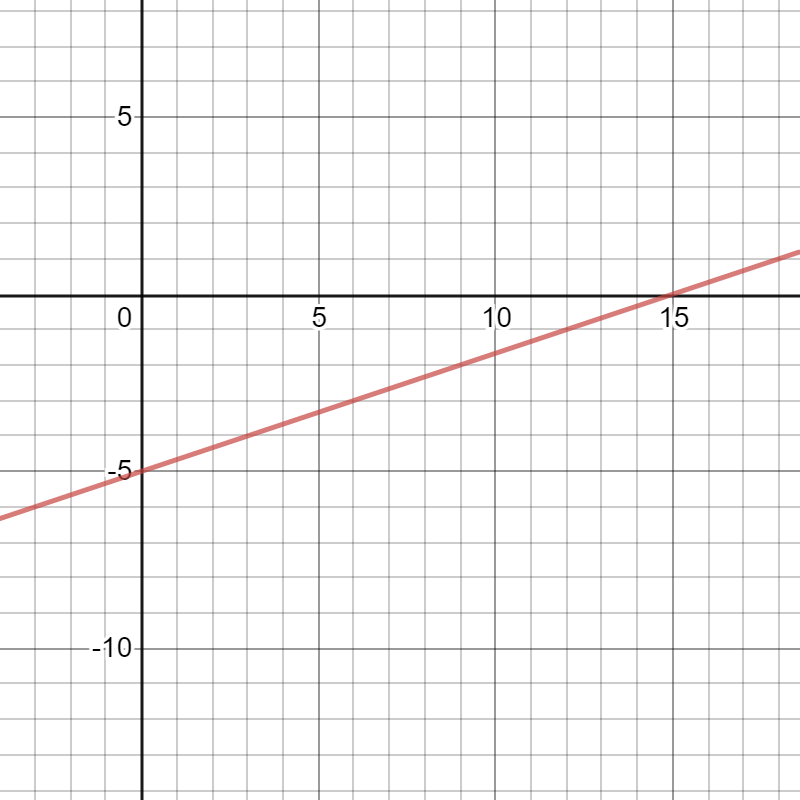
\includegraphics[scale=0.25]{desmos-graph.png}\\

$y=-2x^{2}+7x$

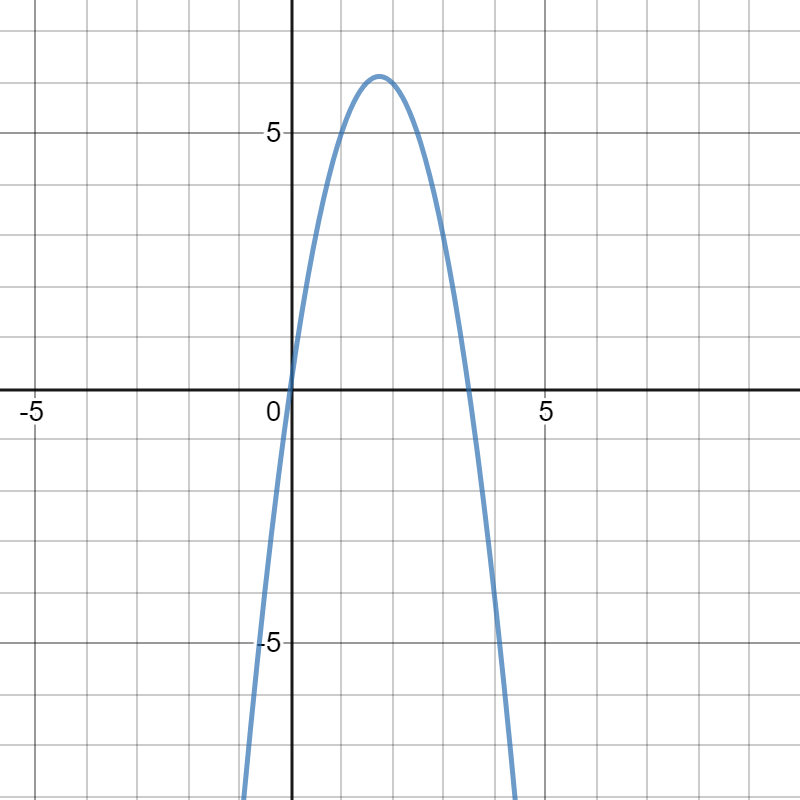
\includegraphics[scale=0.25]{desmos-graph (1).png}\\

\newpage
$f\left(x\right)\ =\ \sqrt{x}-2$

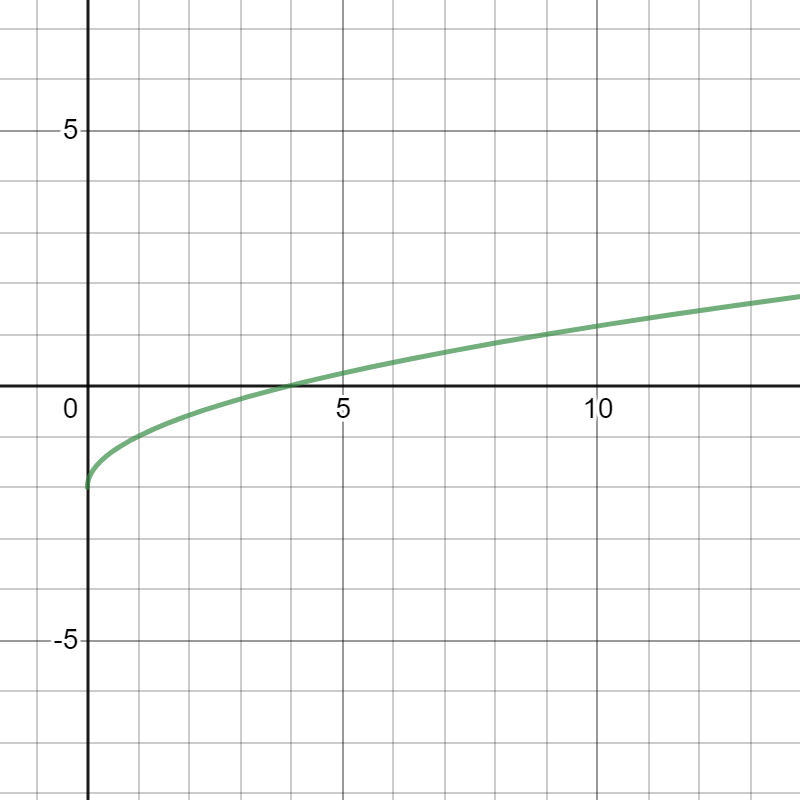
\includegraphics[scale=0.25]{desmos-graph (2).png}\\

$g\left(z\right)=z^{-2}-3z$

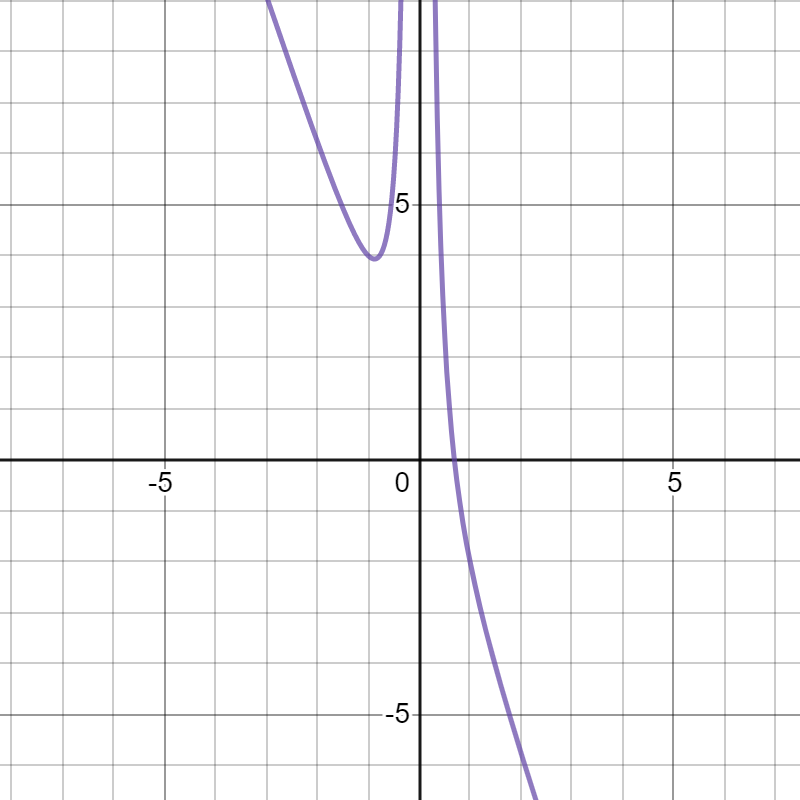
\includegraphics[scale=0.25]{desmos-graph (3).png}\\

\newpage
$y=2x^{3}+3x^{2}-12x+4$

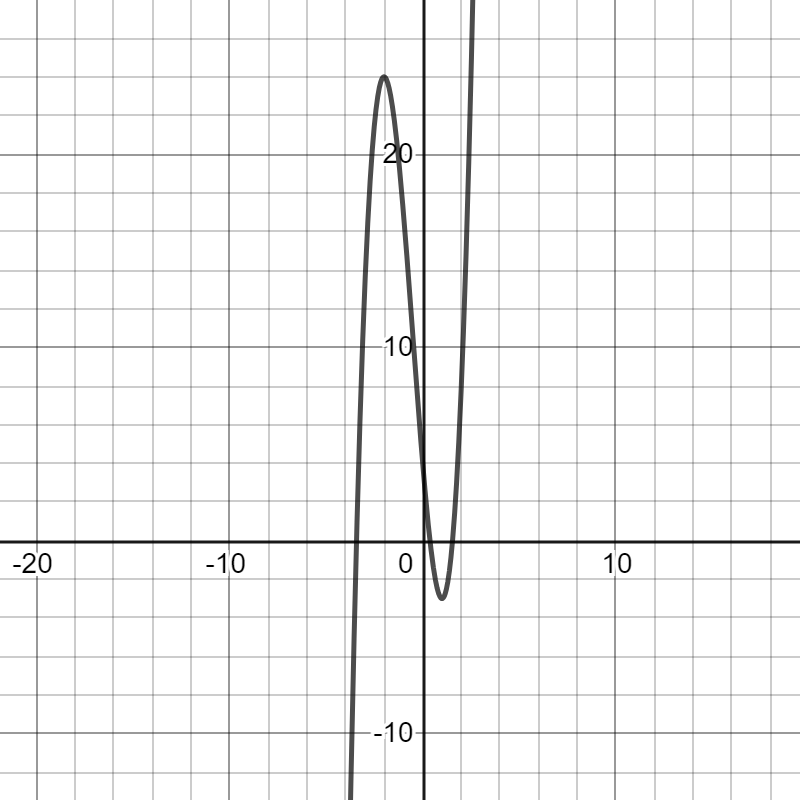
\includegraphics[scale=0.25]{desmos-graph (4).png}


\end{document}